\documentclass[a4paper,11pt]{exam}
%\printanswers % pour imprimer les réponses (corrigé)
\noprintanswers % Pour ne pas imprimer les réponses (énoncé)
%\addpoints % Pour compter les points
% \noaddpoints % pour ne pas compter les points
%\qformat{\textbf{\thequestion ) } }
%\qformat{\textbf{\thequestion )}} % Pour définir le style des questions (facultatif)
\usepackage{color} % définit une nouvelle couleur
\shadedsolutions % définit le style des réponses
% \framedsolutions % définit le style des réponses
\definecolor{SolutionColor}{rgb}{0.8,0.9,1} % bleu ciel
\renewcommand{\solutiontitle}{\noindent\textbf{Solution:}\par\noindent} % Définit le titre des solutions
\usepackage{gensymb}



\makeatletter

\def\maketitle{{\centering%
	\par{\huge\textbf{\@title}}%
	\par{\@date}%
	\par}}


\renewcommand{\thesubsection}{\Alph{subsection}.}   

\makeatother

\lhead{NOM Pr\'enom :}
\rhead{\textbf{Les r\'eponses doivent \^etre justifi\'ees et r\'edig\'ees}}
\cfoot{\thepage / \pageref{LastPage}}


%\usepackage{../../pas-math}
%\usepackage{../../moncours}


%\usepackage{pas-cours}
%-------------------------------------------------------------------------------
%          -Packages nécessaires pour écrire en Français et en UTF8-
%-------------------------------------------------------------------------------
\usepackage[utf8]{inputenc}
\usepackage[frenchb]{babel}
%\usepackage{numprint}
\usepackage[T1]{fontenc}
%\usepackage{lmodern}
\usepackage{textcomp}
\usepackage[french, boxed]{algorithm2e}
\usepackage{hyperref}


%-------------------------------------------------------------------------------

%-------------------------------------------------------------------------------
%                          -Outils de mise en forme-
%-------------------------------------------------------------------------------
\usepackage{hyperref}
\hypersetup{pdfstartview=XYZ}
%\usepackage{enumerate}
\usepackage{graphicx}
\usepackage{multicol}
\usepackage{tabularx}
\usepackage{multirow}
\usepackage{color}
\usepackage{eurosym}


\usepackage{anysize} %%pour pouvoir mettre les marges qu'on veut
%\marginsize{2.5cm}{2.5cm}{2.5cm}{2.5cm}

\usepackage{indentfirst} %%pour que les premier paragraphes soient aussi indentés
\usepackage{verbatim}
\usepackage{enumitem}
\usepackage{booktabs}
\usepackage[usenames,dvipsnames,svgnames,table]{xcolor}

\usepackage{variations}

%-------------------------------------------------------------------------------


%-------------------------------------------------------------------------------
%                  -Nécessaires pour écrire des mathématiques-
%-------------------------------------------------------------------------------
\usepackage{amsfonts}
\usepackage{amssymb}
\usepackage{amsmath}
\usepackage{amsthm}
\usepackage{tikz}
\usepackage{xlop}
\usepackage[output-decimal-marker={,}]{siunitx}
%-------------------------------------------------------------------------------

%-------------------------------------------------------------------------------
%                  -Nécessaires pour écrire des formules chimiquess-
%-------------------------------------------------------------------------------

\usepackage[version=4]{mhchem}

%-------------------------------------------------------------------------------
% Pour pouvoir exploiter les fichiers directement dans beamer
\newcommand{\pause}{\ }
%-------------------------------------------------------------------------------
%                    - Mise en forme avancée
%-------------------------------------------------------------------------------

\usepackage{ifthen}
\usepackage{ifmtarg}


\newcommand{\ifTrue}[2]{\ifthenelse{\equal{#1}{true}}{#2}{$\qquad \qquad$}}

%\newcommand{\kword}[1]{\textcolor{red}{\underline{#1}}}
%-------------------------------------------------------------------------------

%-------------------------------------------------------------------------------
%                     -Mise en forme d'exercices-
%-------------------------------------------------------------------------------
%\newtheoremstyle{exostyle}
%{\topsep}% espace avant
%{\topsep}% espace apres
%{}% Police utilisee par le style de thm
%{}% Indentation (vide = aucune, \parindent = indentation paragraphe)
%{\bfseries}% Police du titre de thm
%{.}% Signe de ponctuation apres le titre du thm
%{ }% Espace apres le titre du thm (\newline = linebreak)
%{\thmname{#1}\thmnumber{ #2}\thmnote{. \normalfont{\textit{#3}}}}% composants du titre du thm : \thmname = nom du thm, \thmnumber = numéro du thm, \thmnote = sous-titre du thm

%\theoremstyle{exostyle}
%\newtheorem{exercice}{Exercice}
%
%\newenvironment{questions}{
%\begin{enumerate}[\hspace{12pt}\bfseries\itshape a.]}{\end{enumerate}
%} %mettre un 1 à la place du a si on veut des numéros au lieu de lettres pour les questions 
%-------------------------------------------------------------------------------

%-------------------------------------------------------------------------------
%                    - Mise en forme de tableaux -
%-------------------------------------------------------------------------------

\renewcommand{\arraystretch}{1.7}

\setlength{\tabcolsep}{1.2cm}

%-------------------------------------------------------------------------------



%-------------------------------------------------------------------------------
%                    - Racourcis d'écriture -
%-------------------------------------------------------------------------------
%Droites
\newcommand{\dte}[1]{$(#1)$}
\newcommand{\fig}[1]{figure $#1$}
\newcommand{\sym}{symétrique}
\newcommand{\syms}{symétriques}
\newcommand{\asym}{axe de symétrie}
\newcommand{\asyms}{axes de symétrie}
\newcommand{\seg}[1]{$[#1]$}
\newcommand{\monAngle}[1]{$\widehat{#1}$}
\newcommand{\bissec}{bissectrice}
\newcommand{\mediat}{médiatrice}
\newcommand{\ddte}[1]{$[#1)$}


% Angles orientés (couples de vecteurs)
\newcommand{\aopp}[2]{(\vec{#1}, \vec{#2})} %Les deuc vecteurs sont positifs
\newcommand{\aopn}[2]{(\vec{#1}, -\vec{#2})} %Le second vecteur est négatif
\newcommand{\aonp}[2]{(-\vec{#1}, \vec{#2})} %Le premier vecteur est négatif
\newcommand{\aonn}[2]{(-\vec{#1}, -\vec{#2})} %Les deux vecteurs sont négatifs

%Ensembles mathématiques
\newcommand{\naturels}{\mathbb{N}} %Nombres naturels
\newcommand{\relatifs}{\mathbb{Z}} %Nombres relatifs
\newcommand{\rationnels}{\mathbb{Q}} %Nombres rationnels
\newcommand{\reels}{\mathbb{R}} %Nombres réels
\newcommand{\complexes}{\mathbb{C}} %Nombres complexes


%Intégration des parenthèses aux cosinus
\newcommand{\cosP}[1]{\cos\left(#1\right)}
\newcommand{\sinP}[1]{\sin\left(#1\right)}


%Probas stats
\newcommand{\stat}{statistique}
\newcommand{\stats}{statistiques}


\newcommand{\homo}{homothétie}
\newcommand{\homos}{homothéties}


\newcommand{\mycoord}[3]{(\textcolor{red}{\num{#1}} ; \textcolor{Green}{\num{#2}} ; \textcolor{blue}{\num{#3}})}
%-------------------------------------------------------------------------------

%-------------------------------------------------------------------------------
%                    - Mise en page -
%-------------------------------------------------------------------------------

\newcommand{\twoCol}[1]{\begin{multicols}{2}#1\end{multicols}}


\setenumerate[1]{font=\bfseries,label=\textit{\alph*})}
\setenumerate[2]{font=\bfseries,label=\arabic*)}


%-------------------------------------------------------------------------------
%                    - Elements cours -
%-------------------------------------------------------------------------------

%Correction d'exercice
\newcommand{\exoSec}[2]{\subsection*{Exercice #1 page #2}}
%-------------------------------------------------------------------------------
%                    - raccourcis d'écriture -
%-------------------------------------------------------------------------------

%Mise en évidence de termes clés
\newcommand{\mykw}[1]{\textcolor{red}{\underline{\textbf{#1}}}}

%Exercices
\newcommand{\exo}[2]{exercice #1 page #2}
\newcommand{\Exo}[2]{Exercice #1 page #2}

\renewcommand{\pause}{\ }

%Intervalles
\newcommand{\interOO}[2]{$]$#1 , #2$[$}
\newcommand{\interOF}[2]{$]$#1 , #2$]$}
\newcommand{\interFO}[2]{$[$#1 , #2$[$}
\newcommand{\interFF}[2]{$[$#1 , #2$]$}



%\usepackage{fullpage}
\author{\ }
\date{4 Février 2019}
\title{Sciences Physiques : DS n° 4}


\begin{document}
%	\usepackage{fancyhdr}
%	
%	\pagestyle{fancy}
%	\fancyhf{}
	%\rhead{Share\LaTeX}

	\maketitle
	
\begin{small}
	\begin{center}
		\begin{tabular}{|@{\ }l@{}|@{\ }c@{\ }|}
			\hline
			\textbf{Compétence} & \textbf{Maitrise} \\
			\hline
			Changements d’états de la matière \ &  \ \ \ \\
			\hline
			Conservation de la masse, variation du volume, température de changement d’état \ &  \ \ \ \\
			\hline
		\end{tabular}
	\end{center}
\end{small}	
	
	
%\vspace*{-0.5cm}	

%\section{\'Equations de réaction}

Ajuster les équations de réactions suivantes :
\begin{questions}
	\question $CH_4 + ....O_2 \rightarrow ....CO_2 + ....H_2O$
	
	\question $C_7H_{16} + ....O_2 \rightarrow ....CO_2 + ....H_2O$	
	
	\question $C_6H_{2}O + ....O_2 \rightarrow ....CO_2 + ....H_2O$
\end{questions}


%\section{À chaque modèle sa formule}
\begin{questions}
	\question \'A partir de ces dessins de modèles, donner la formule des molécules suivantes.

	\begin{center}
		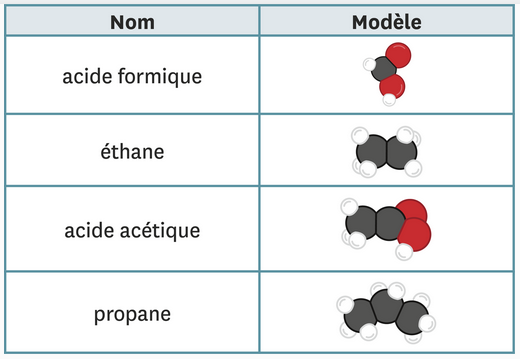
\includegraphics[scale=0.6]{img/exemples}
	\end{center}
	\fillwithdottedlines{2cm}
	
\end{questions}

%Seul l'\ref{ex:surface} est à faire sur le sujet.
Le soin et la qualité de rédaction sont pris en compte dans la notation.


%\section{Quels atomes dans cette particule ? (4 points)}\label{ex:particule}



\begin{questions}
	\question[4] Pour chaque espèce chimique, indiquer le type d'atome, le nombre d'atomes de chaque type et le nombre total d'atomes qu'elle contient.
	 
	\begin{multicols}{4}
		\begin{itemize}
			\item $CO_2$
			\item $H_2$
			\item $CH_4$
			\item $O_2$
			\item $C_4H_{10} $
			\item $C_6H_{12} O_6$
			\item $C$
			\item $H_2O$
		\end{itemize}
	\end{multicols}

	\begin{solution}
		\begin{tabular}{|@{\ }c@{\ }|@{\ }c@{\ }|@{\ }c@{\ }|@{\ }c@{\ }|@{\ }c@{\ }|}
			\hline
			Molécule         & Nombre d'atomes & Nombre d'atomes & Nombre d'atomes & Nombre total \\ 
			& de carbone      & d'hydrogène     & d'oxygène       & d'atomes         \\ \hline
			$CO_2$           & 1               & 0               & 2               & 3               \\ \hline
			$H_2$            & 0               & 2               & 0               & 2               \\ \hline
			$CH_4$           & 1               & 4               & 0               & 5               \\ \hline
			$O_2$            & 0               & 0               & 2               & 2               \\ \hline
			$C_4H_{10}$      & 4               & 10              & 0               & 14              \\ \hline
			$C_6H_{12}O_{6}$ & 6               & 12              & 6               & 24              \\ \hline
			$C$              & 1               & 0               & 0               & 1               \\ \hline
			$H_2O$           & 0               & 2               & 1               & 3               \\ \hline
		\end{tabular}
	\end{solution}
	
\end{questions}

%\newpage




%\section{La phrase mystère (2 points)}

Construire une phrase expliquant ce qui se passe dans le compartiment à glace d'un réfrigérateur lorsqu'on fabrique des glaçons, en utilisant les expressions suivantes :

\begin{multicols}{3}
	\begin{itemize}
		\item se solidifie
		\item cède de l'énergie
		\item l'eau liquide
		\item à l'air
		\item température de 0°C
	\end{itemize}
\end{multicols}

%\section{Brouillard : gaz ou liquide ?}

Alexandre fait chauffer de l'eau pour faire cuire des pâtes. Quand l'eau arrive à ébullition, il passe rapidement sa main dans le <<brouillard>> au-dessus de la casserole.

Expliquer pourquoi la main d'Alexandre est alors humide ?
\section{Volume d'une piscine}

Pierre veut installer une piscine dans son jardin mais il ne veut pas utiliser plus de 45 $m^3$ d'eau pour la remplir. Il a sélectionné un modèle avec les dimensions suivantes : longueur = 8 m, largeur = 5 m, hauteur 150 cm.

\begin{questions}
	\question Calculer le volume de la piscine sélectionnée.
	\begin{solution}
	\end{solution}
	
	\question Pierre peut-il choisir ce modèle de piscine ?
	\begin{solution}
		
	\end{solution}
\end{questions}

\section{Précision de la verrerie (4 points)}

Voici deux instruments de mesure :

\begin{center}
	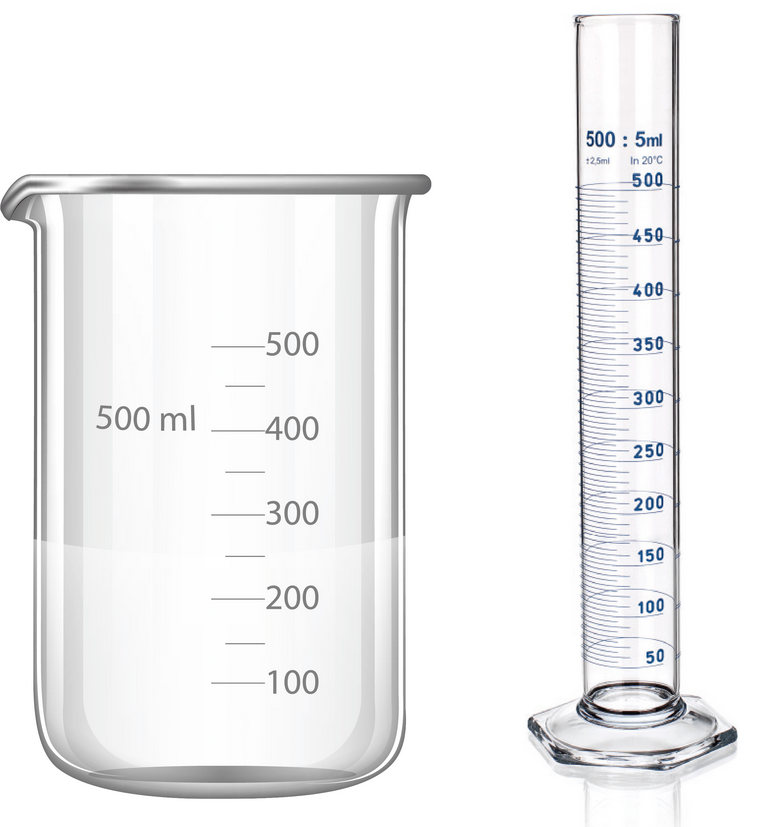
\includegraphics[scale=0.4]{img/vol}
\end{center}

\begin{questions}
	\question[1] Quel est leur nom ?

		\begin{solution}
			
		\end{solution}
	
	\question[1] Quelle est l'unité de mesure utilisée pour ces instruments de mesure ?

	\question[1] Dans chaque cas, à quel volume correspond un intervalle ?
	
	%\question[1] Si l'on se trompe d'une graduation, quelle sera l'erreur commise sur la mesure ?
	
	\question[1] Lequel de ces instruments permet d'effectuer la masure la plus précise ?
	
%	\question Existe-t-il une relation entre le diamètre de l'instrument de mesure et la précision des mesures ?

\end{questions} 

\newpage

\section{Mesurer un volume }\label{ex:temperture}


\begin{questions}
	
	\begin{multicols}{2}
		
	
		\question[] Quel volume maximal, en cm3, peut-on mesurer avec chacune des éprouvettes ci-contre ?
		
		\question[]	Quel est le volume de liquide contenu dans chacune des éprouvettes ?
		
		\begin{center}
			
		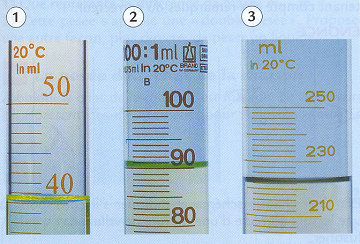
\includegraphics[scale=0.8]{img/mesure1}
		\end{center}
		
	\end{multicols}
	
\end{questions}


\section{Volume de billes (4 points)}


\begin{multicols}{2}
	

Noémie place des billes dans une éprouvette graduée.

\begin{questions}
	\question[1] Quelle est la valeur $V_1$ du volume du tas de billes dans l'éprouvette ? 
	
	\question[1\half] Elle verse de l'eau dans une éprouvette identique à la précédente. Puis elle verse l'eau dans l'éprouvette contenant les billes. Quel est le volume $V_2$ occupé par les billes ?
	
	\question[1\half] Comment expliquer la différence entre le volume $V_1$ et le volume $V_2$.
\end{questions}


\begin{center}
	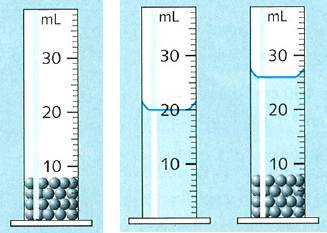
\includegraphics[scale=0.9]{img/billes}
\end{center}
\end{multicols}


 


\section{L'or de Max (5 points)}

Max dispose d'un lot de 12 pièces de collection et souhaite vérifier qu'elles sont en or pur. Il a lu dans son livre de Physique que 1 $dm^3$ d'or avait une masse de \num{19.3} $kg$. Il possède une éprouvette graduée de 100 $mL$ et une balance. Il sait que :

\begin{itemize}
	\item 1 $dm^3$ de plomb a une masse de \num{11.34} $kg$;
	\item 1 $dm^3$ de nickel a une masse de \num{8.9} $kg$;
\end{itemize} 
\begin{questions}
	\question[1] Quelles grandeurs Max doit-il mesurer afin de vérifier le métal dont les pièces sont faites.
	\begin{solution}
		Max doit mesurer la masse et le volume de ses pièces.
	\end{solution}
	
	\question[1] Expliquer pourquoi c'est mieux de mesurer le volume d'au moins 10 pièces en même temps dans l'éprouvette graduée.
	\begin{solution}
		Le volume d'une pièce est proche de la précision de l'éprouvette, en mesurant le volume de 10 pièce on aura une mesure plus précise.
	\end{solution}
	
	\question[1] 10 pièces ont un volume $V = 14\; mL$ et la masse d'une pièce est $m  = \num{12,46}\; g$. Calcule la masse de 1 $dm^3$ de pièces.
	\begin{solution}
		1 pièce a une masse de $\num{12,46}\; g$, donc 10 pièces auront une masse de $\num{124,6}\; g$. soit $\num{0,1246}\; kg$. Ces 1à pièces occupent $14 mL$ soit $\num{0.014} L$ donc $\num{0.014} dm^3$ .
		
		\begin{equation*}
			\num{0,1246} \div \num{0.014} = \num{8.9}
		\end{equation*}
		
		1 $dm^3$ de pièce a donc une masse de \num{8.9} kg.
	\end{solution}


	\question[1] Les pièces de Max sont-elles en or ?
	\begin{solution}
		$\num{8.9} \neq \num{19.3}$, donc les pièces ne sont pas en or.
	\end{solution}
	
	\question[1] Dans quel métal sont elles faites ?
	\begin{solution}
		Ces pièces ont une masse volumique de $\num{8.9} kg/dm^3$, elles sont donc en nickel.
	\end{solution}
\end{questions}


\ \label{LastPage}

\end{document}